%
% Sección de diseño,
% Análisis y diseño de tienda en línea
% Proyecto Lovelace
%

\section{Diseño}
En esta sección se incluyen los aspectos del diseño del caso de prueba
librería en línea.

\subsection{Diseño de la base de datos}
En la figura \ref{lib_fig:relacional} se encuentra el diagrama relacional de
la base de datos.

\begin{figure}
  \begin{center}
    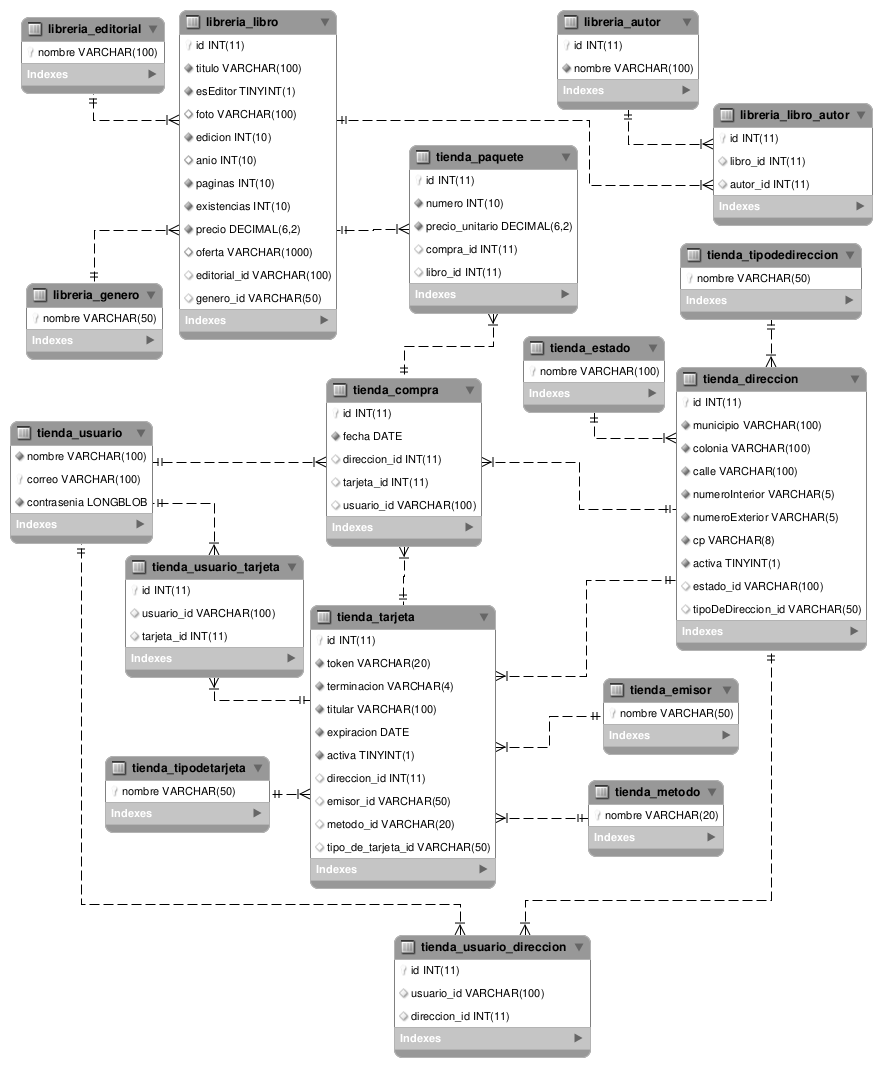
\includegraphics[width=1.0\linewidth]{diagramas/relacional.png}
    \caption{Diagrama relacional de la base de datos.}
    \label{lib_fig:relacional}
  \end{center}
\end{figure}

\subsection{Vista dinámica}
Comenzando con los diagramas de secuencia para algunos de las acciones, en la
figura~\ref{lib_fig:secuencia_registrar_cliente} se muestra el correspondiente
para el proceso de registrar a un cliente en la tienda en línea (para más
detalles, véase \hipervinculo{lib_cu:registrar_cliente}); en la
figura~\ref{lib_fig:secuencia_agregar_libro_al_carrito}, el diagrama para
agregar un libro al carrito; finalmente, en~\ref{lib_fig:secuencia_comprar},
se observa la secuencia para realizar una compra.

\begin{figure}
  \begin{center}
    \subimport{diagramas/}{secuencia_registrar_cliente.tikz.tex}
    \caption{Diagrama de secuencia para registrar a un cliente.}
    \label{lib_fig:secuencia_registrar_cliente}
  \end{center}
\end{figure}

\begin{figure}
  \begin{center}
    \subimport{diagramas/}{secuencia_agregar_libro_al_carrito.tikz.tex}
    \caption{Diagrama de secuencia para agregar un libro al carrito.}
    \label{lib_fig:secuencia_agregar_libro_al_carrito}
  \end{center}
\end{figure}

\begin{sidewaysfigure}
  \begin{center}
    \subimport{diagramas/}{secuencia_comprar.tikz.tex}
    \caption{Diagrama de secuencia para realizar una compra.}
    \label{lib_fig:secuencia_comprar}
  \end{center}
\end{sidewaysfigure}
